\section{Results} \label{sec4}

After carrying out carefully the data preprocessing, feature engineering and training steps, we have obtained the trained classifier. In this section we are going to present the results of the training. 

\subsection{Model Evaluation and Validation}

After validating by overfitting to a single training example that the model is implemented correctly and is able to learn we carried out a hyperparameter search in the parameter space. The hyperparameters were chosen with which the highest validation accuracy was acquired. These parameters are provided in section \ref{sec3.4}. The model was then fully trained with these parameters. The training and validation loss during training can be examined in Figure \ref{fig12}

\begin{figure}[h]
	\centering
	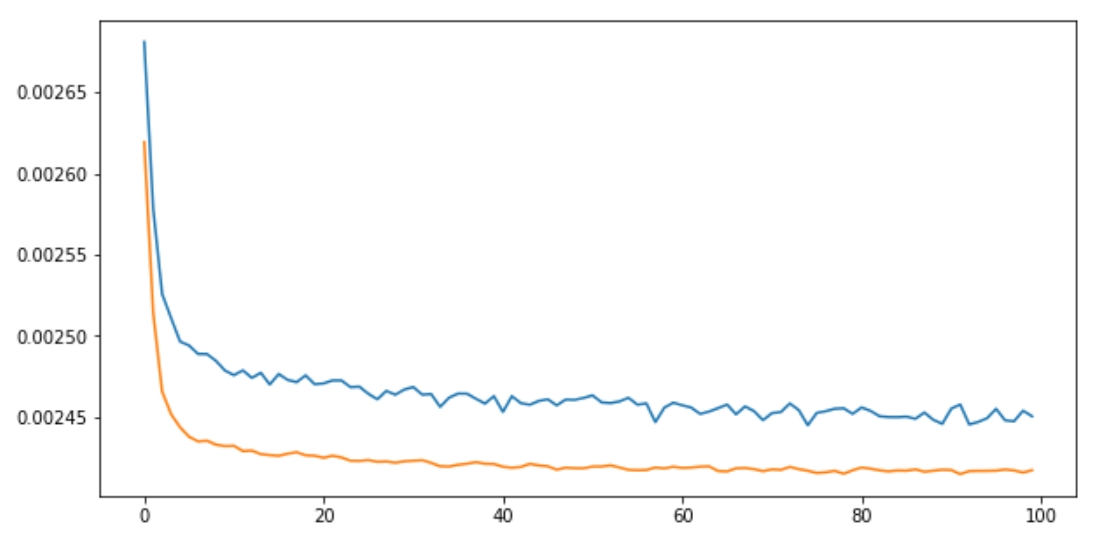
\includegraphics[width=0.7\textwidth]{fig/loss.jpg}
	\vspace*{-0.1in}
	\caption{Training (blue) and validation (orange) loss during training.}
	\label{fig12}
	\vspace*{-0.2in}
	\bigskip
\end{figure}

From this figure one can conclude that the training has converged to a local optima. The regularization is also sufficient as the model does not overfit to the data. (Does not memorizes the labels of the training set.) The phenomena that the validation loss is smaller than the training loss is thanks to the regularization technique. Since dropout is only used during training and is switched off during validation, the validation loss becomes lower during training. 

After training, the model was evaluated on the test set which was never shown to the model before. On the test set the model was able to reach an accuracy of 52\%. 

The benchmark model was also evaluated with different number of neighbors. It was able to produce an accuracy of 46\% with k=10 neighbors. 

Hence we conclude that the trained neural network was able to outperform the kNN classifier slightly. Further analysis and justification of the results is provided in the next subsection.


\subsection{Justification}

The successfully trained model was tested on the test set which was never seen before. It acquired 52\% accuracy on this set. This is a slight improvement compared to the accuracy of the benchmark kNN classifier (46\%). 

Although this accuracy does not seem to be very high, let us place it into context. We have also expected a somewhat higher accuracy than this number. 52\% accuracy means that only in slightly more than half of the cases the future of a received offer were predicted successfully. In other words, the classifier is only able to predict the reaction of every second costumer. 

However one have to consider the following properties of the situation to be able to evaluate the performance in its context. First of all, the received offers are classified into 4 classes. This means that a random classifier would achieve an accuracy around 25\%. Our classifier has reached an accuracy more than twice as high. Also a very important aspect that one has to keep in mind is how dynamically change the behavior of the people. It really is a stochastic environment. It is totally possible, that someone have completed a certain offer 5 out of 5 times before and still does not completes it the $6^{th}$ time. People behave so stochastically that it is impossible to tell their reaction to certain offers with a very high accuracy. 

In this respect we conclude that although this accuracy is not very high, it is still a surprisingly good result considering the complexity and randomness of the task it solves. Being able to predict the exact outcome of an advertising campaign for every second person could be a very powerful tool for companies such as Starbucks.

\subsection{Summary}

In this report we have detailed our solution for Starbuck's Capstone Challenge. Our chosen aim was to try to predict, into which of the following four classes a received offer is going to fall given some basic data about the person who receives the offer and its costumer history until receiving the offer.:

\begin{itemize}
	\item Will not be viewed nor completed accidentally
	\item Will not be viewed but will be completed
	\item Will be viewed but will not be completed
	\item Will be completed and viewed
\end{itemize}

We have explored the provided data thoroughly, identified the issues with it and provided solutions to remedy them. We have preprocessed the dataset to make it sufficiently well behaving for training and developed a feature representation which from our point of view describes the costumers and their costumer history until receiving the offer accurately. We have extracted the features from the raw dataset and created the corresponding labels.

We have implemented a feed forward neural network for the above classification purpose. After searching the sufficient hyperparameters, we have trained the network with the training data. We then compared its results with our benchmark model, which is a kNN classifier with 10 neighbors.

We have reached an accuracy of 52\% on the testing set, which is a slight improvement on the kNN classifier which have reached 46\%. Although these accuracy numbers do not seem to be very high, considering the randomness on how people act in the real word, these numbers are quite impressive in our point of view. For every second person one is able to predict exactly what the future of an offer is going to be. 

This can be a powerful tool for companies. Considering the accuracy of the model, a useful application of such a model would be to check the success of a campaign for a large number of costumers and obtain whether for most of the people it would be successful or not. 


\subsection{Outlook}

After training the model, we have also trained an other network for a slightly different purpose. We have re-classified the received offers only into successful and not successful categories. We considered the offers to be successful if they were viewed and completed or if they were plain informational offers and they were viewed. We have trained a neural network with the same features for this binary classification task. 

We were able to obtain the following results with it:
\begin{itemize}
	\item accuracy: 65\%
	\item precision: 49\%
	\item recall: 75\%
	\item false negative rate: 25\%
\end{itemize}

From these measures the high recall and low false negative rate are especially appealing. This means that the model mostly classifies successful outcomes correctly and most of the failures are made by classifying some offers to be successful although they will not be successful in fact. This is the smaller problem. A bigger problem would be if customers who would otherwise not receive the offer do not receive the offer at all.

In this respect a further improvement in this direction could be an interesting field of further research.














